\chapter{Methodology}
\label{mt:methodology}

In this section, we will walk through all the organizational aspects related to the project: configuration management, \gls{ci}/\gls{cd} workflows, micro-service architecture structure and model definition.

\section{Configuration Management}

Configuration management can be defined as a process that ensures the consistency and quality of a project/product through its life cycle and the various changes it undergoes. Sometimes the term is mistaken for version control, but in fact configuration management includes version control.

In this subsection we will talk about the different technologies and tools that have been used in order to keep a decent control of configuration management.

\subsection{Git \& GitHub}

As mentioned above, version control is a part of configuration management and is responsible for recognizing and managing the various changes of software code. Version control systems are software tools that help teams manage changes to source code over time. 

For this project Git has been the clear option since it is the market leader due to its huge speed and its branch and merge functionality, among others. Taken from its website \enquote{Git is a free and open source distributed version control system designed to handle everything from small to very large projects with speed and efficiency}.~\cite{gitDefinition}

GitHub is essentially a remote repository hosting platform for Git. It allows developers to work together on the same project from anywhere. Figure~\ref{fig:current-status-github} presents an example.

\begin{figure}[H]
    \centering
    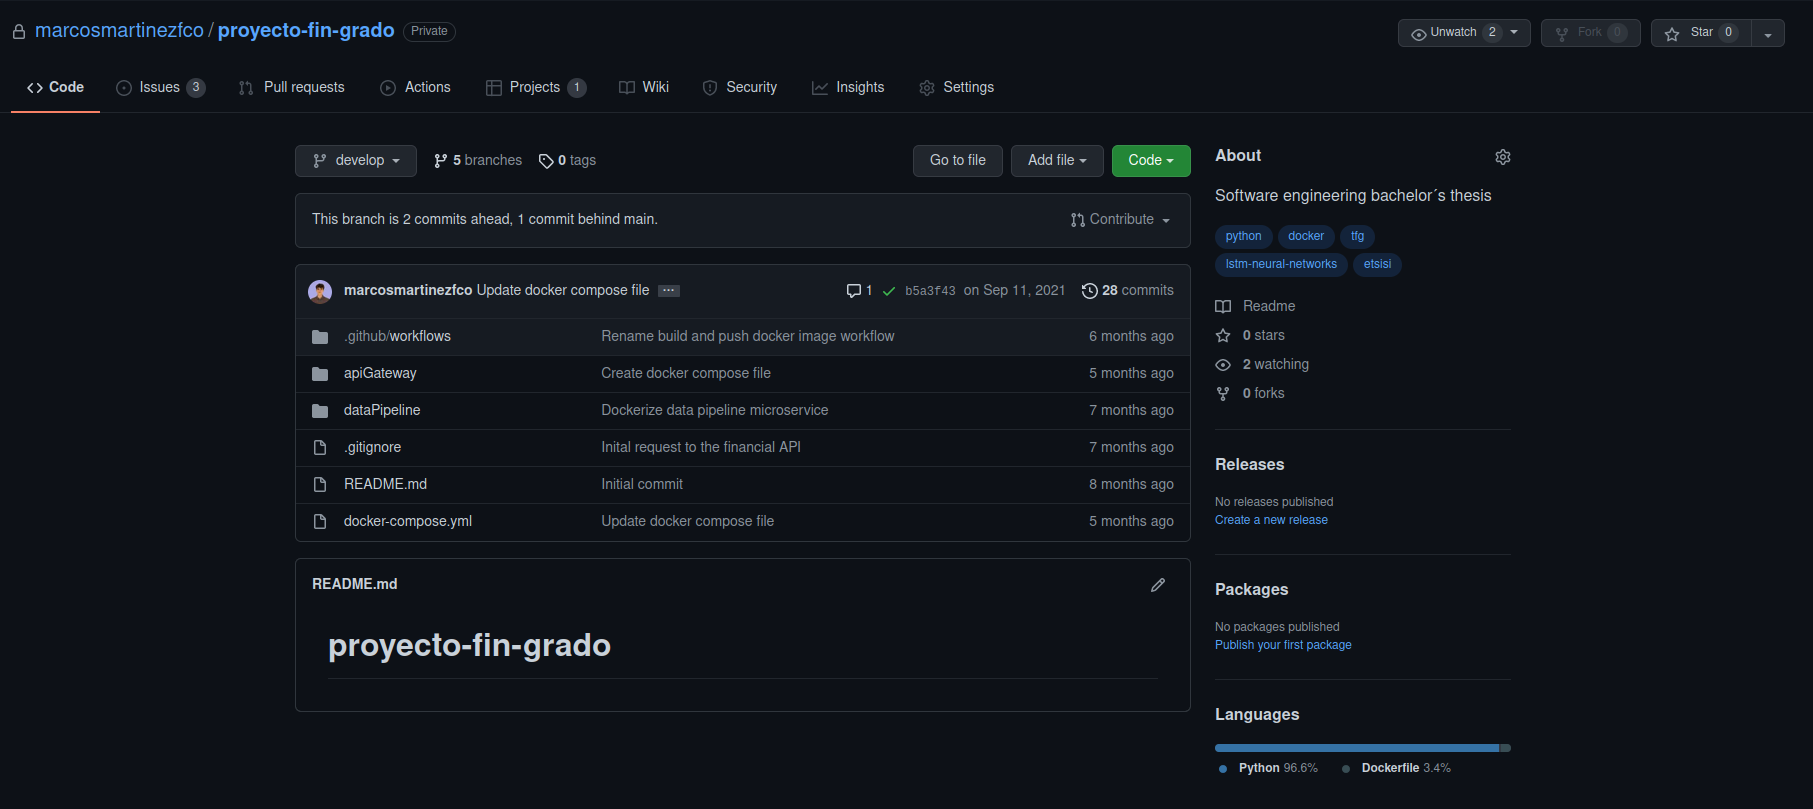
\includegraphics[width=\textwidth]{figures/github.png}
    \caption{GitHub Repository}
    \label{fig:current-status-github}
\end{figure}

\subsection{Git Workflow}

A Git workflow is a template for how to use git to accomplish work in a consistent and productive manner. Git is extremely flexible when it comes to managing changes, so there is no imposed or standardized process. When working with a team on a project, it is important to make sure that the entire team is familiar with how changes will be applied. 

Gitflow has been chosen for this project because of its versatility and the ability to generate branches for each of the features needed for the project, Figure~\ref{fig:gitflow-example}. In our case, it will be extremely useful to be able to develop each of the modules/micro-services of the system in parallel.

\begin{figure}[H]
    \centering
    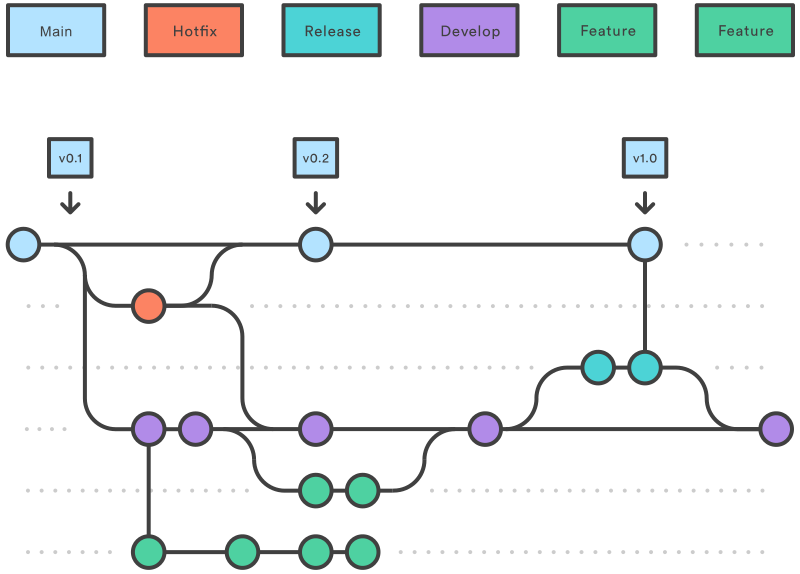
\includegraphics[width=0.55\textwidth]{figures/gitflow.png}
    \caption{Gitflow Scheme, Source: www.atlassian.com~\cite{gitflow}}
    \label{fig:gitflow-example}
\end{figure}

\subsection{GitHub Projects}

When planning a project, one of the most important tasks is the identification and organization of the necessary work to do in order to complete the project. Due to the changing nature of a degree's thesis and all its uncertainties, agile methodologies seem to be the clear choice to organize its planning and be able to adapt to any change or problem that may appear during its different stages. For this specific thesis different agile methodologies have been used to enhance its development, among which sprints~\footnote{Short, time-boxed period when a scrum team works to complete a set amount of work.~\cite{sprintsDef}} and \gls{Kanban} boards~\footnote{Agile project management tool designed to help visualize work, limit work-in-progress, and maximize efficiency.~\cite{kanbanDef}} stand out.

GitHub provides a helpful tool for creating and managing \gls{Kanban} boards called projects. Figure~\ref{fig:github-projects} shows a snapshot of my project backlog. Task can be either added, edited or deleted from the backlog. They can also be transferred among stages and you can even link them to pull requests or issues which is extremely convenient for workflow automation, since tasks can be automatically transferred around depending on the outcome of those issues/pull requests.

As for the sprints, every two weeks I would meet with my mentor to review the status of the project and discuss about the next steps to take. After that, all the decisions were reflected on the backlog hosted in the GitHub projects, until the end of the newly started sprint.

\begin{figure}[h]
    \centering
    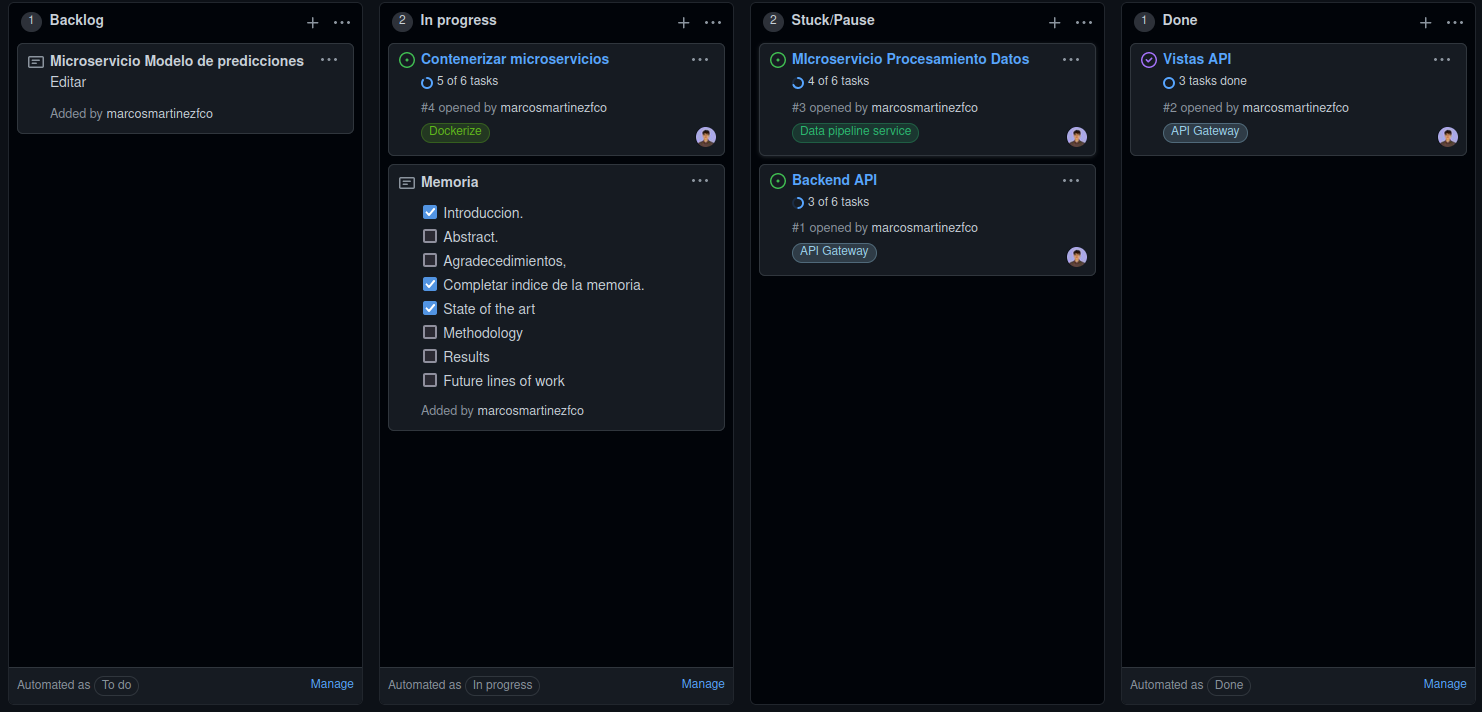
\includegraphics[width=\textwidth]{figures/github-projects.png}
    \caption{Github Projects Kanban}
    \label{fig:github-projects}
\end{figure}

\section{CI/CD Workflows}

One of the main goals during the design phase of this thesis is to have a high level of automation to be able to maintain all the different development processes related to micro-services. Luckily GitHub provides us with a powerful tool for creating custom workflow pipelines, called GitHub actions. These workflows must be located in a folder called \textbf{.github/workflows}, in the root of the repository in different "YAML" files.

GitHub actions fees depend on computing time and the runner's \gls{os}. Runners are responsible for executing the different jobs specified in a workflow, Tab~\ref{tab:action-fees} shows the different prices.

\begin{table}[h]
\centering
\caption{Runner Fees}
\label{tab:action-fees}
\begin{tabular}{@{}ll@{}}
\toprule
Linux             & \$0.008/min \\ \midrule
Windows           & \$0.016/min \\ \midrule
macOs             & \$0.08/min  \\ \midrule
Self-hosted       & Free        \\ \midrule
Public repository & Free       
\end{tabular}
\end{table}

\subsection{Self-hosted Runner}

\begin{lstlisting}[language=bash, caption=Set up Self-hosted Runner,label={lst:self-hosted-runner}]
$ curl -o actions-runner-linux-x64-2.287.1.tar.gz -L https://github.com/actions/runner/releases/download/v2.287.1/actions-runner-linux-x64-2.287.1.tar.gz
$ tar xzf ./actions-runner-linux-x64-2.287.1.tar.gz
$ ./config.sh --url https://github.com/username/repository --token "YOUR TOKEN"
$ ./run.sh
$ sudo ./svc.sh install #this will create a systemd daemon to start the runner on start up
\end{lstlisting}

Self-hosted runners offer more control of hardware, \gls{os}, and software tools than GitHub-hosted runners provide. With self-hosted runners, you can choose to create a custom hardware configuration with more processing power or memory to run larger jobs, install software available on your local network, and choose an \gls{os} not offered by GitHub-hosted runners. Self-hosted runners can be physical, virtual, in a container, on-premises, or in a cloud~\cite{selfHostedRunner}.

To add a self-hosted runner, is as simple as going to the actions section in the repository settings and follow the instructions, Listing~\ref{lst:self-hosted-runner} shows the steps used to configure a Linux based runner for the project. From now on, our self-hosted runner will listen for jobs from our GitHub repository and start executing them whenever a workflow is triggered.

\subsection{Workflow Definition}

Two of the most important aspects to take into consideration when defining a workflow, are the branches or events that will trigger it and the jobs and tasks to be executed. Note that these jobs do not necessarily have to be sequentially executed, in fact they run in parallel by default. Nonetheless, GitHub actions allows us to establish dependencies between jobs, so that certain ones are executed before others.

Triggering events must be defined under the \enquote{on}: tag. Listing~\ref{lst:trigger-options} shows an example of a couple of interesting ones, for more information about triggering events follow the instructions in the action's documentation.

\begin{lstlisting}[caption=Common Workflow Triggers,label={lst:trigger-options}]
on:
  push:
    branches: [only when specific branches are pushed]
    branches-ignore: [ignored branches]
    paths: # triggers when a push to specific files occurs
        - '**.sol'
  pull_request:
    types: [pull request activity type]
  workflow_dispatch: # allows the workflow to be triggered manually
\end{lstlisting}

As for the job definition, they all must be declared under the \enquote{job} tag. Jobs run in parallel by default as we explained before. To run them sequentially, you can define dependencies as Listing~\ref{lst:jobs-definition} shows. Also, the runner which will execute the job, needs to be chosen in the definition.

\begin{lstlisting}[caption=Job Dependencies Definition,label={lst:jobs-definition}]
jobs:
  jobA:
    runs-on: [self-hosted] # the job will be forwarded to our self-hosted runner
  jobB:
    runs-on: [ubuntu-latest] # the job will be executed in a hosted ubuntu machine
    needs: jobA
  jobC:
    runs-on: [self-hosted]
    if: ${{ always() }} #jobC will execute regardless of jobA & jobB output
    needs: [jobA, jobB]
\end{lstlisting}

The most powerful feature about GitHub actions is the integration with its whole ecosystem. So for instance, each job has a list of steps which are always executed sequentially and they all need to pass, in order for the job to successfully finish. These task can be either manually specified or reused from the Action's marketplace, where everyone can either upload or reuse published actions. To use any of them, is as simple as specifying the dependency \enquote{publisher/actions@version}. Listing~\ref{lst:step-definition} shows an example of a reused action from the marketplace.

Another useful feature is the \enquote{secrets} environment, which lets you define repository level environment variables that need to be off the code, i.e, \gls{api} keys, tokens or cryptography private keys.

\begin{lstlisting}[caption=Steps Definition,label={lst:step-definition}]
steps:
- uses: actions/first-interaction@v1 # dependency definition
  with:
    repo-token: ${{ secrets.GITHUB_TOKEN }} # GitHub environment variable
    issue-message: 'message that will be displayed on users' first issue'
    pr-message: 'message that will be displayed on users' first pr'
\end{lstlisting}

\subsection{Build \& Push Workflow}

As shown in Listing~\ref{lst:build-push-docker}, \enquote{Build-push-docker-images.yml} describes the workflow used for building and pushing the different docker images used in the project into docker hub. Automating all code deployment generated during development.

\begin{lstlisting}[caption=build-push-docker-images.yml,label={lst:build-push-docker}]
name: Build an push docker images to docker hub
on:
  push:
    branches: [main , develop]
  workflow_dispatch:
jobs:
  build:
    runs-on: self-hosted
    steps:
      - name: Repo checkout
        uses: actions/checkout@v2
      - name: Docker Login
        uses: docker/login-action@v1.10.0
        with:
          username: ${{secrets.DOCKER_USERNAME}}
          password: ${{secrets.DOCKER_TOKEN}}
      - name: Build and push api-gateway image
        uses: docker/build-push-action@v2
        with:
          context: apiGateway/
          push: true
          tags: marcosmartinezfco/tfg-api-gateway:latest
      - name: Build and push data-pipeline image
        uses: docker/build-push-action@v2
        with:
          context: dataPipeline/
          push: true
          tags: marcosmartinezfco/tfg-data-pipeline:latest
\end{lstlisting}

\section{Micro-service Architecture}
\label{Micro-service Architecture}

In section~\ref{Micro-services Architecture} we introduced the micro-service architecture pattern and its features. This section will focus in the different technologies that have been used to implement the pattern and the general layout of the application.

\begin{figure}[h]
    \centering
    \caption{Architecture Layout}
    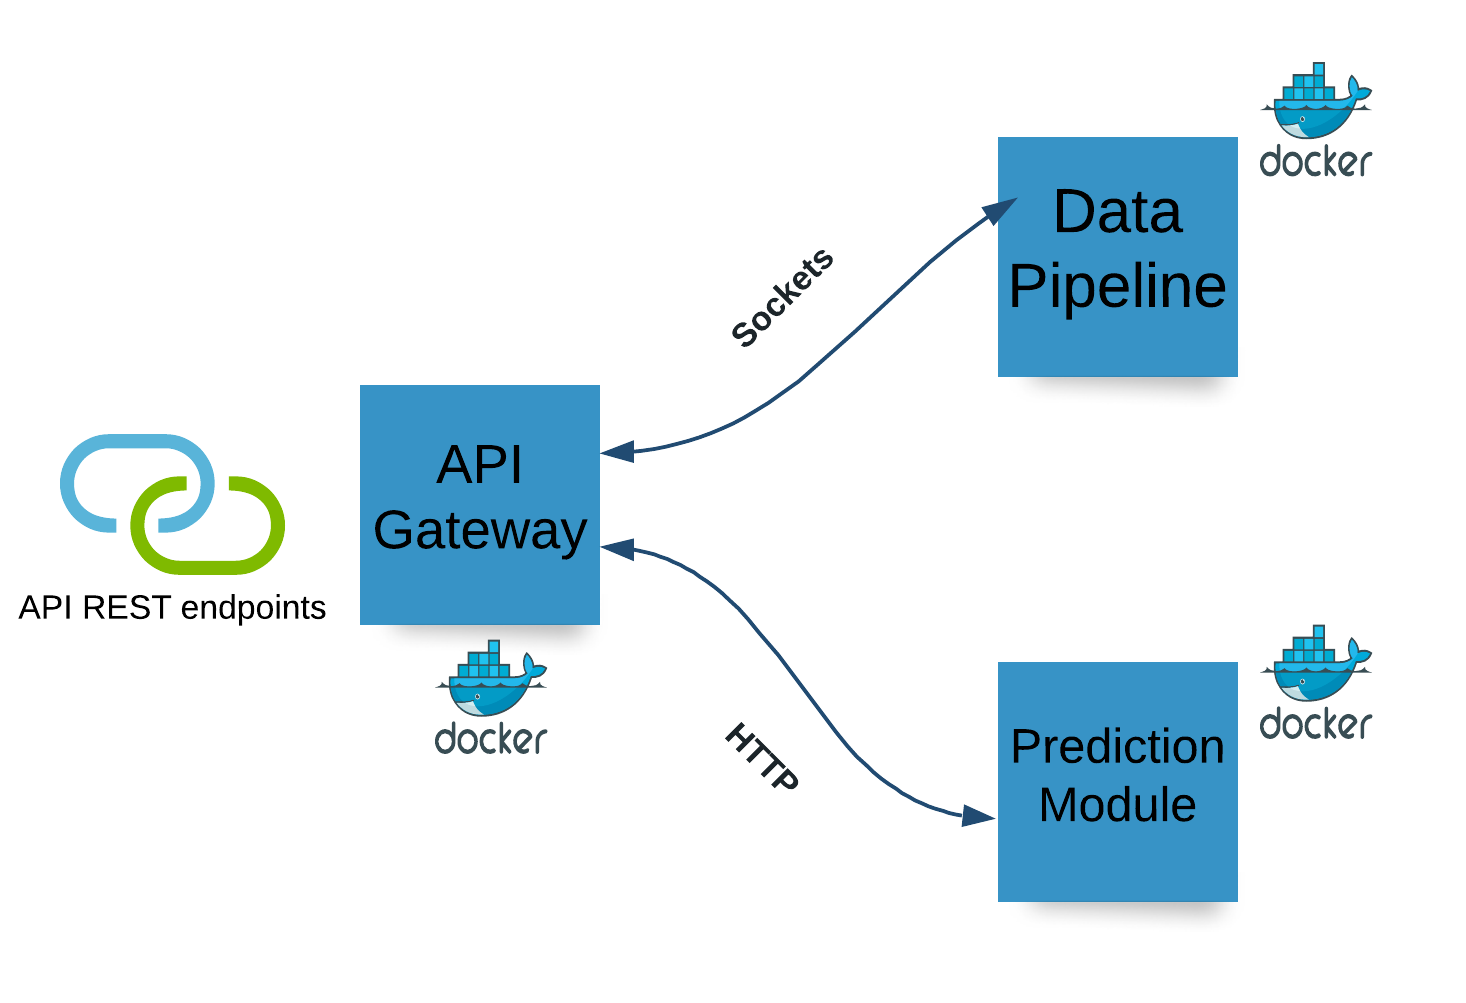
\includegraphics[width=\textwidth]{figures/architecture.png}
    \label{fig:architecture-layout}
\end{figure}

Figure~\ref{fig:architecture-layout} shows all the micro-services the architecture is decomposed into, each of which is an independent docker container as we previously have mentioned:

\begin{itemize}
    \item \gls{api} Gateway is the module that provides the endpoints users will use to get the predictions.
    \item Data pipeline is the module in charge of downloading the historical data of an asset which will be fed to the model in order to get the prediction for that asset.
    \item The prediction module is in charge of receiving a time-series with historical data of a company and then forecasting a prediction of the closing price. We will be using the battle tested tool Tensorflow Serve to implement this micro-service.
\end{itemize}

\subsection{Container communication}
\label{Container communication}

 Given the fact that containers act as an isolated system from the host and seeing Figure~\ref{fig:architecture-layout}, a natural question arise. How do these containers communicate with one another?
 
 One of the main reasons for Docker popularity is containers and services do not even need to be aware that they are deployed on Docker, or the host's \gls{os}, or whether their peers are also Docker workloads or not. You can use Docker to manage containers in a platform-agnostic way through Docker networking drivers~\cite{dockerNetworking}. These drivers allow you to specify how containers should behave and communicate, as Table~\ref{tab:docker-drivers} shows.
 
\begin{table}[h]
\centering
\caption{Docker Network Drivers}
\label{tab:docker-drivers}
\begin{tabular}{@{}|c|l|@{}}
\toprule
\textbf{Driver} & \multicolumn{1}{c|}{\textbf{Funcitonality}}                                                                                            \\ \midrule
Bridge          & \begin{tabular}[c]{@{}l@{}}Is best when you need multiple\\ containers to communicate on the same host.\end{tabular}                   \\ \midrule
Host            & \begin{tabular}[c]{@{}l@{}}Removes network isolation between \\ the container and the host, using its networking directly.\end{tabular} \\ \midrule
Overlay &
  \begin{tabular}[c]{@{}l@{}}Is best when you need containers running on \\ different hosts to communicate. It connects multiple Docker \\ daemons together, removing the need to do OS-level routing.\end{tabular} \\ \midrule
macVLAN &
  \begin{tabular}[c]{@{}l@{}}Allows you to assign a MAC address to a container,\\ making it appear as a physical device on your network.\end{tabular} \\ \midrule
Custom          & Third-party network plugins.                                                                                                           \\ \midrule
None            & It disables all networking, usually used together with a custom driver.                                                                \\ \bottomrule
\end{tabular}
\end{table}

This project uses the bridge driver since the host machine houses all the orchestration. On their own, bridge networks provide a software networking layer which allows connected containers to communicate, while providing full isolation from containers that are not connected.

Docker creates a bridge network by default to which all containers are connected if not specified otherwise. These containers can reference one another based on their IP address. User-defined networks can also be created, with the advantage of more configuration capabilities and containers being able to reference one another by their name instead of an IP address. Fig~\ref{fig:tfg-net} shows the user-defined bridge network used in this project.

\begin{figure}[h]
    \centering
    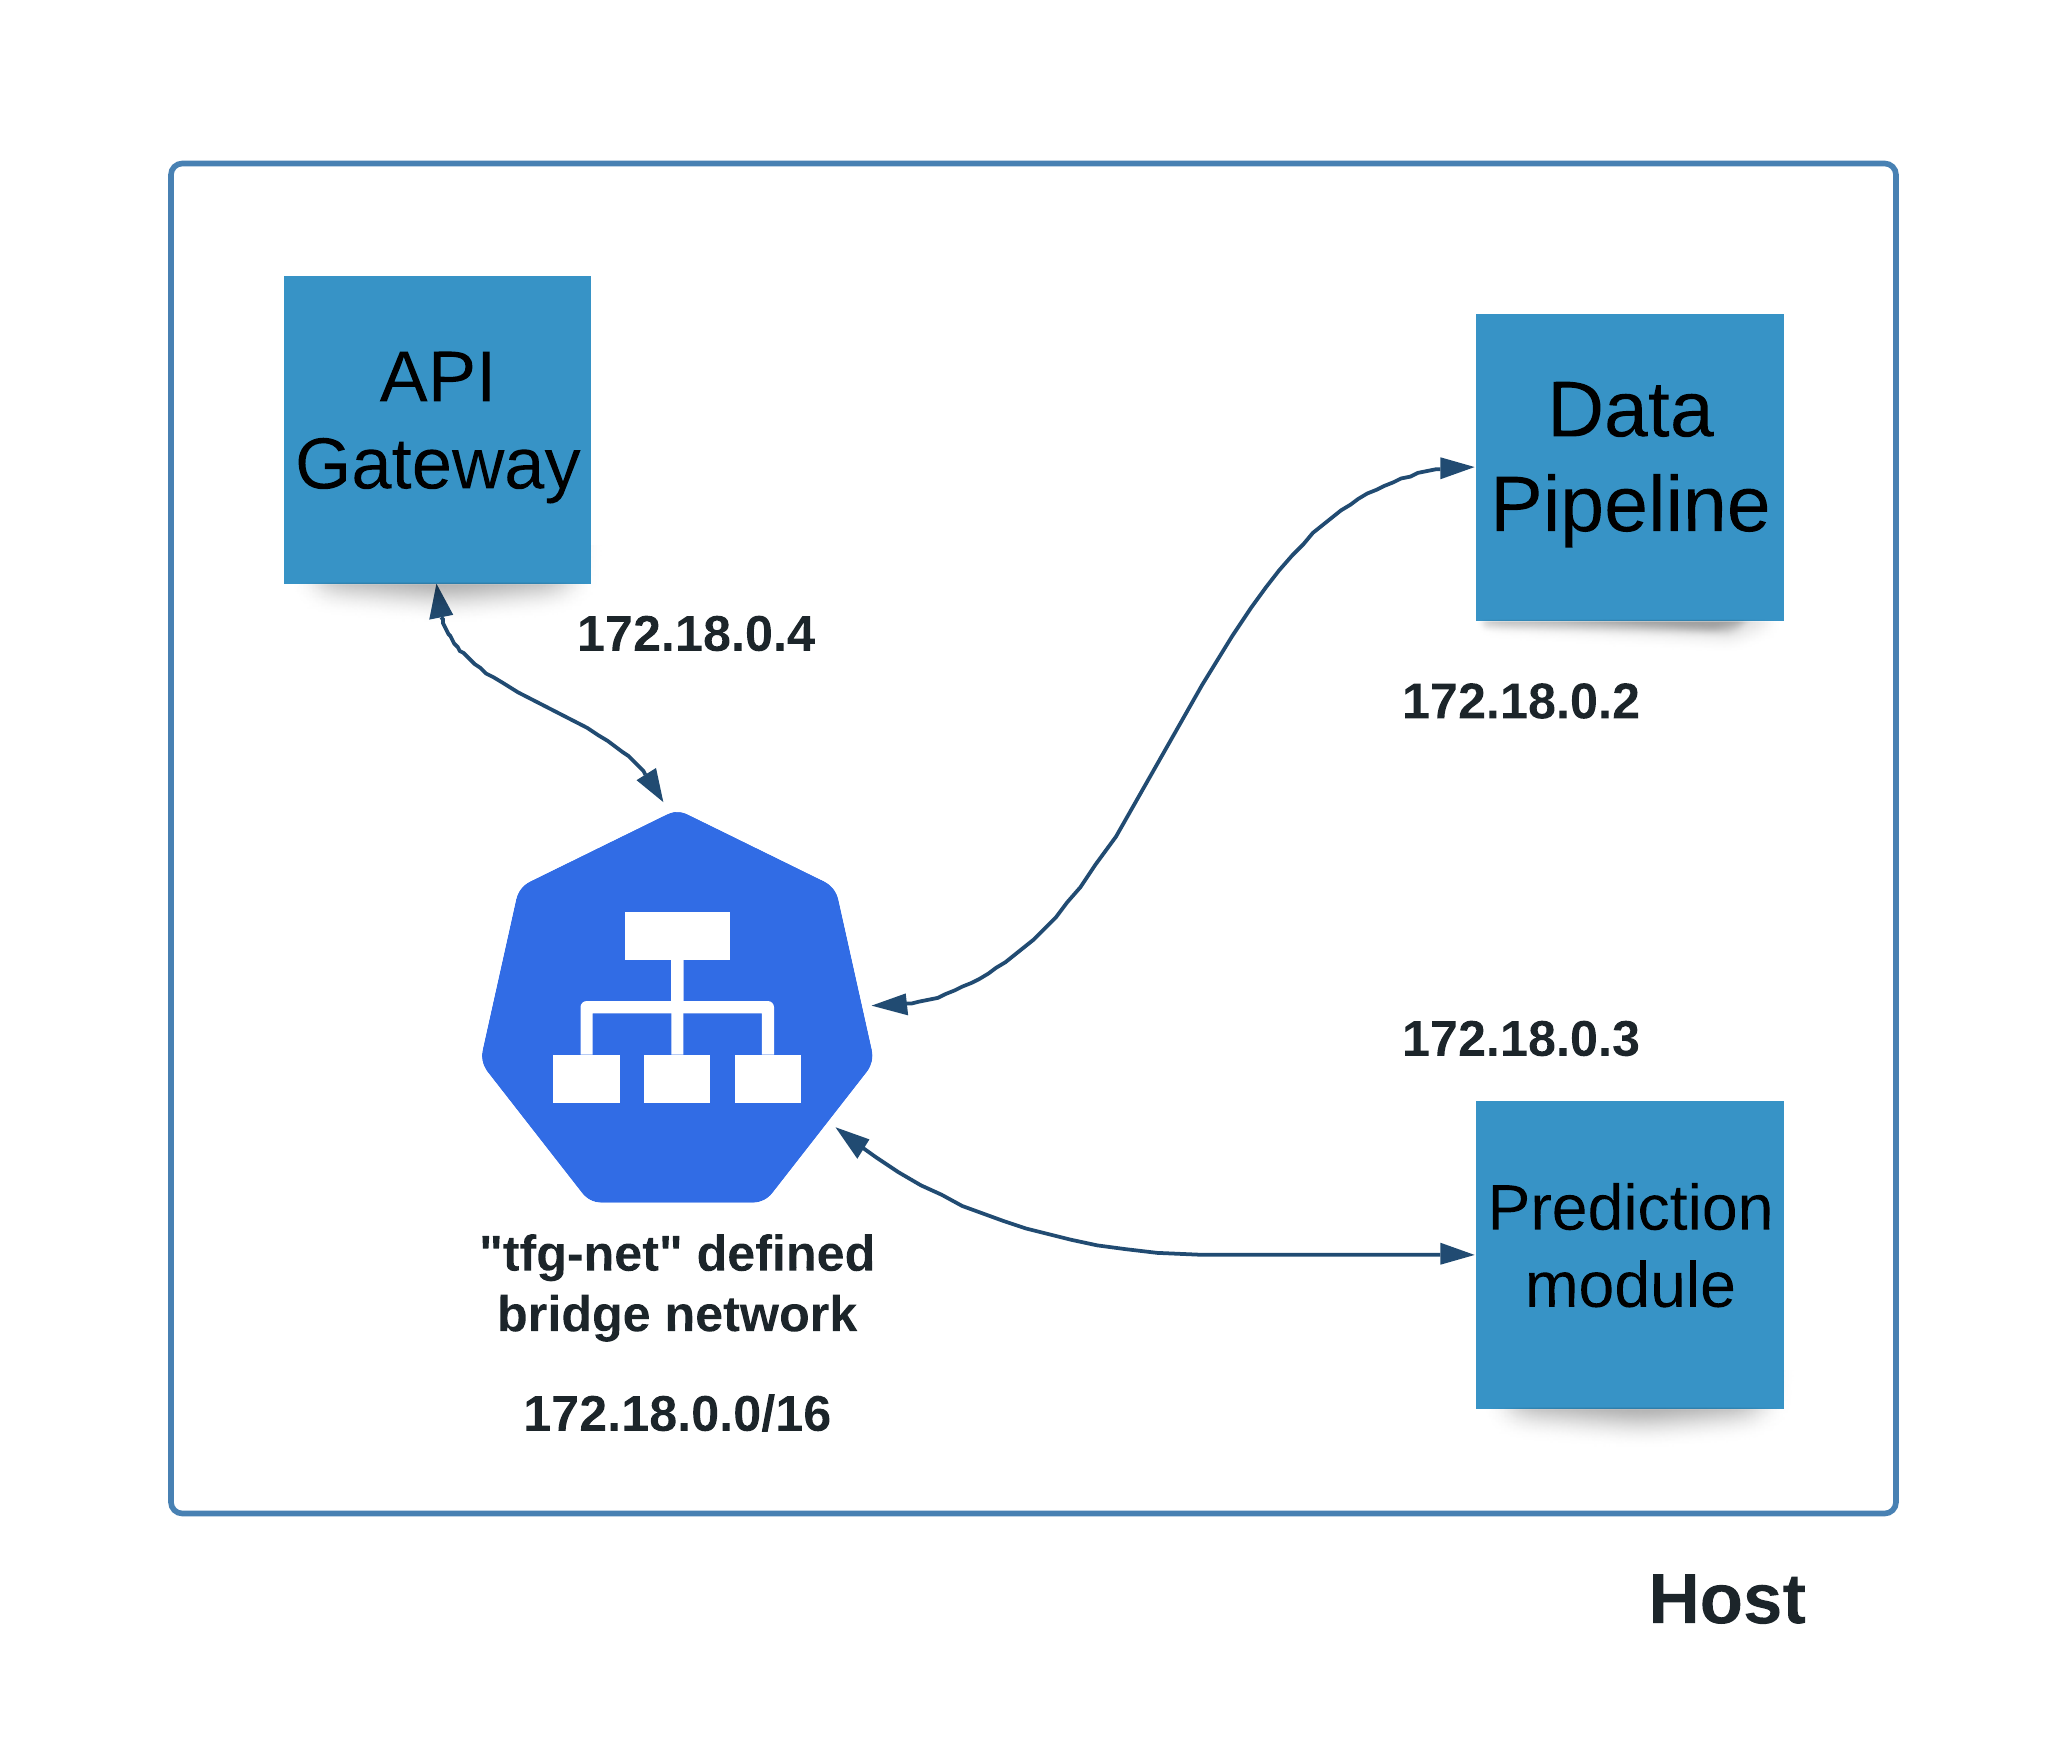
\includegraphics[width=\textwidth]{figures/tfg-net.png}
     \caption{User Defined Network}
    \label{fig:tfg-net}
\end{figure}

Communication will take place between two defined channels, the first one between $"API Gateway \longleftrightarrow Data Pipeline"$ and the second one between $"API Gateway \longleftrightarrow Prediction Module"$. In both scenarios, the Data Pipeline module and the Prediction module act as the server and the \gls{api} Gateway as the client requesting a service. 

Regarding the Python standard library for sockets connections, for sending data we find the \lstinline[language=python]{sendall()} function. This function unlike \lstinline[language=python]{send()}, continues to send data until either it all has been sent or an error occurs. None is returned on success. On the other hand, due to packet fragmentation a custom implementation of \lstinline[language=python]{receive()} is needed to make sure all the response data is being received, since the standard library does not support this feature. Listing~\ref{lst:receive-all} shows the custom implementation of \lstinline[language=python]{receiveall()}, notice that all the data sent or received through the socket must be byte encoded.\\

\begin{lstlisting}[language=python,caption=Custom Implementation receiveall(),label={lst:receive-all}]
def receive_all(conn: socket) -> bytes:
    # first we receive a header containing the length of the data
    msg_len = recv_header(conn)
    data = b''
    while len(data) < msg_len:
        packet = conn.recv(msg_len - len(data))
        if not packet:
            break
        data += packet
    return data
\end{lstlisting}

\subsection{API Gateway}

As shown in Figure~\ref{fig:architecture-layout}, the main function of the \gls{api} Gateway is to provide the \gls{RESTful} endpoints users will interact with to obtain their predictions. To satisfy user requests, the Gateway will forward these petitions. First to the Data Pipeline module, which will respond with the historical data of the requested company. Second, after receiving the response It will launch a request to the Prediction module, from which the final price prediction of the requested company will be received. Finally, the \gls{api} Gateway serves the user's original request by returning a \gls{json} file either with the prediction or an error message.

There are several Python frameworks to work with \glspl{api} but \gls{Django} has been the final option due to its market popularity and wide community support, even thought for this project a simpler option like Flask would have been more than enough.

The first step to build our \gls{api} endpoints is to create a new application, which will wrap our micro-service logic, inside our blank Django project in the \textbf{\enquote{projectName/settings.py}} module, as Listing~\ref{lst:settings.py} shows. After creating the application, we need to tell Django to forward all incoming petitions to the newly created app, Listing~\ref{lst:root/urls.py}, as it will take care of all the logic.\newpage

\begin{lstlisting}[language=python,caption=apiGateway/settings.py,label={lst:settings.py}]
# Application definition
INSTALLED_APPS = [
    'django.contrib.admin',
    'django.contrib.auth',
    'django.contrib.contenttypes',
    'django.contrib.sessions',
    'django.contrib.messages',
    'django.contrib.staticfiles',
    'rest_framework', #we add this powerful toolkit for building APIs
    'restApi.apps.RestapiConfig', #points to the restApi config file
]
\end{lstlisting}

\begin{lstlisting}[language=python,caption=apiGateway/urls.py,label={lst:root/urls.py}]
urlpatterns = [
    path('admin/', admin.site.urls),
    # we forward all incoming petitions to the respApi app urls.py module
    path('', include('restApi.urls')) 
]
\end{lstlisting}

\begin{lstlisting}[language=python,caption=restApi/urls.py,label={lst:restApi/urls.py}]
urlpatterns = [
    #forward the petitions to a class based view
    path('prediction/<str:ticker>/', views.PredictionView.as_view()),
]
\end{lstlisting}

Now all petitions are being routed to our application, but we need to specify an endpoint for users to communicate with our service. In Listing~\ref{lst:restApi/urls.py} we create the only endpoint our \gls{api} will recognize, \textbf{\enquote{/prediction/<str:ticker>}}. The last part of the url, \textbf{\enquote{<str:ticker>}}, allows us to serialize the company ticker\footnote{An abbreviation used to uniquely identify publicly traded shares of a particular stock on a particular stock market.}, so that it is passed as a parameter to the corresponding view.

Now that we are capable of routing petitions we need to create a view, which is a Python function or class that takes a web request and returns a web response, to manage them. Two types of views are built-in in the Django framework, function views and class based views, which need to be declared inside the \textbf{\enquote{restApi/views.py}} module. For this project the class based view has been the final option simply because each single \gls{http} request method can be defined by a matching name function, as Listing~\ref{lst:restApi/views.py} shows.

\begin{lstlisting}[language=python,caption=restApi/views.py,label={lst:restApi/views.py}]
class PredictionView(APIView):
    """
    Class based view for all the nasdaq related requests
    """
    def get(self, request, ticker: str):
        client = Client(os.getenv('PIPELINE_IP', 'data-pipeline'), 15032)
        data = client.connect(ticker)
        raw_df = pd.DataFrame(json.loads(data)["Time Series (Daily)"]).T
        for c in raw_df.columns:
            raw_df[c] = pd.to_numeric(raw_df[c])
        raw_df.index = pd.to_datetime(raw_df.index)
        response = requests.post('http://prediction-module:8501/v1/models/{model}:predict', data=json.dumps({
            "signature_name": "serving_default",
            "instances":  raw_df.sort_index().iloc[-1].to_numpy().reshape(1, 5).tolist()
        }))
        return JsonResponse(response.json())
\end{lstlisting}

In section~\ref{Container communication} we explained how containers communicated among one another and that the API Gateway always acted as a client, either to request data to the Data Pipeline module or to the Predcition module as seen in Listing~\ref{lst:restApi/views.py}. Listing~\ref{lst:restApi/client.py} shows the implementation of the client class for communicating with Data Pipeline module using sockets.

\begin{lstlisting}[language=python,caption=restApi/client.py,label={lst:restApi/client.py}]
class Client:
    FORMAT = 'utf-8'
    BUFFER_SIZE = 4096
    HEADER = 64

    def __init__(self, server_ip: str, port: int):
        self.server_ip = server_ip
        self.port = port
        self.server = socket.socket(socket.AF_INET, socket.SOCK_STREAM)

    def connect(self, symbol: str) -> str:
        with self.server as s:
            s.connect((self.server_ip, self.port))
            len_symbol = prepared_send(symbol)
            s.sendall(len_symbol)
            s.sendall(symbol.encode(Client.FORMAT))
            return recv_all(s).decode(Client.FORMAT)

\end{lstlisting}

Last but not least, once we have all the \gls{api} Gateway code implemented, we need to specify \gls{Docker} how to containerize the application so that our build and push workflow in Listing~\ref{lst:build-push-docker} can automatically build and upload the Docker image to Docker Hub. Listing~\ref{lst:ApiGateway-dockerfile} shows the Dockerfile used to create the image to build the container. 


\begin{lstlisting}[language=python,caption=Api Gateway Dockerfile,label={lst:ApiGateway-dockerfile}]
FROM    ubuntu
RUN     apt -y -q update && apt -y -q install python3 python3-pip
COPY    . /api-gateway 
WORKDIR /api-gateway
#install dependencies
RUN     pip3 install -r requirements.txt 
EXPOSE  8000/tcp
ENTRYPOINT ["python3", "manage.py", "runserver", "0.0.0.0:8000"] 
\end{lstlisting}

\subsection{Data pipeline}

\begin{lstlisting}[language=python,caption=aplha-vantage.py,label={lst:alpha-vantage}]
def download_data(symbol: str, function='TIME_SERIES_WEEKLY', dump=False) -> dict:
    valid, best_match = validate_symbol(symbol)
    if not valid:
        return _not_valid(dump)
    url = f'https://www.alphavantage.co/query?function={function}&symbol={best_match}&interval=5min&' \
          F'apikey={API_KEY}'
    r = requests.get(url)
    if dump:
        _dump_data(r.json(), 'api_data.txt')
    return r.json()

def validate_symbol(symbol: str) -> (bool, str):
    url = f'https://www.alphavantage.co/query?function=SYMBOL_SEARCH&keywords={symbol}&apikey={API_KEY}'
    r = requests.get(url)
    matches = r.json().get('bestMatches', None)
    if not matches:
        return False, symbol
    return True, matches[0]['1. symbol']

def _not_valid(dump: bool) -> dict:
    data = {"Error": "No matches found for the requested symbol"}
    if dump:
        _dump_data(data, 'api_data.txt')
    return data

def _dump_data(data: dict, file: str):
    with open(file, 'w') as out:
        json.dump(data, out, sort_keys=True, indent=4)
\end{lstlisting}

The Data Pipeline module's main function, as seen in the architecture layout in Figure~\ref{fig:architecture-layout}, is to wait for petitions, requesting the historical time-series of a given ticker of a company, from the \gls{api} Gateway module. To get the time-series, the Data pipeline module will use the Aplha Vantage \glspl{api}, which provides enterprise-grade financial market data. From traditional asset classes, e.g., stocks and \glspl{etf}, to economic signals, from foreign exchange rates to cryptocurrencies, from fundamental data to technical indicators.~\cite{alphaVantage}

Data from the Alpha Vantage \gls{api} can easily be fetched with the Python package \textbf{\enquote{request}}. Listing~\ref{lst:alpha-vantage} shows the Python implementation to request the data located in the \textbf{\enquote{alpha-vantage.py}} Python module.

In order to be able to respond to requests, we first need to be capable of receiving them. As we mentioned above the Data Pipeline behaves as a server to which the \gls{api} Gateway connects. Listing~\ref{lst:server.py} shows the implementation of the \textbf{\enquote{server.py}} module.

\begin{lstlisting}[language=python,caption=server.py,label={lst:server.py}]
class Server:
    FORMAT = 'utf-8'
    BUFFER_SIZE = 4096
    HEADER = 64

    def __init__(self, addr=None, port=15032):
        if not addr:
            self.addr = socket.gethostbyname(socket.gethostname())
        else:
            self.addr = addr
        self.port = port
        self.server = socket.socket(socket.AF_INET, socket.SOCK_STREAM)

    def start(self):
    """Wait & respond incoming connections"""
        try:
            self.server.bind((self.addr, self.port))
            self.server.listen()
            while True:
                conn, ip = self.server.accept()
                threading.Thread(target=self.manage_client, args=(conn, ip)).start()
        except KeyboardInterrupt:
            self.server.close()

    def manage_client(self, conn: socket, ip: Tuple[str]):
        with conn as c:
            sym_request = recv_all(c).decode(Server.FORMAT)
            self.response_client(sym_request, c)

    def response_client(self, symbol: str, conn: socket):
        data = json.dumps(download_data(symbol))
        encoded_len = prepared_send(data)
        conn.sendall(encoded_len)
        conn.sendall(data.encode(Server.FORMAT))
\end{lstlisting}

As we did in the previous section we need to specify the Dockerfile to build the image. Listing~\ref{lst:dataPipeline-dockerfile} shows the Dockerfile used to create the image to build the container.

\begin{lstlisting}[language=python,caption=Data Pipeline Dockerfile,label={lst:dataPipeline-dockerfile}]
FROM    ubuntu
RUN     apt -y -q update && apt -y -q install python3 python3-pip
COPY    . /alpha-vantage
WORKDIR /alpha-vantage
RUN     mkdir logs
RUN     pip3 install -r requirements.txt
EXPOSE  15032/tcp
ENTRYPOINT ["python3", "main.py"]
\end{lstlisting}

% \notebox{
%     \textbf{"Why do we need to decouple the Data pipeline Module?"}
    
%     After reading this sub-section, you are probably wondering why the Data Pieline module is a container by itself when its logic could just be done inside the \gls{api} Gateway. The main reason besides scalability issues, was to provide a baseline architecture for a future project where more complex data processes  could be applied.
% }

\newpage
\subsection{Prediction module}
\label{prediction-module}

\begin{figure}[h]
    \centering
    \caption{Tensorflow Serving}
    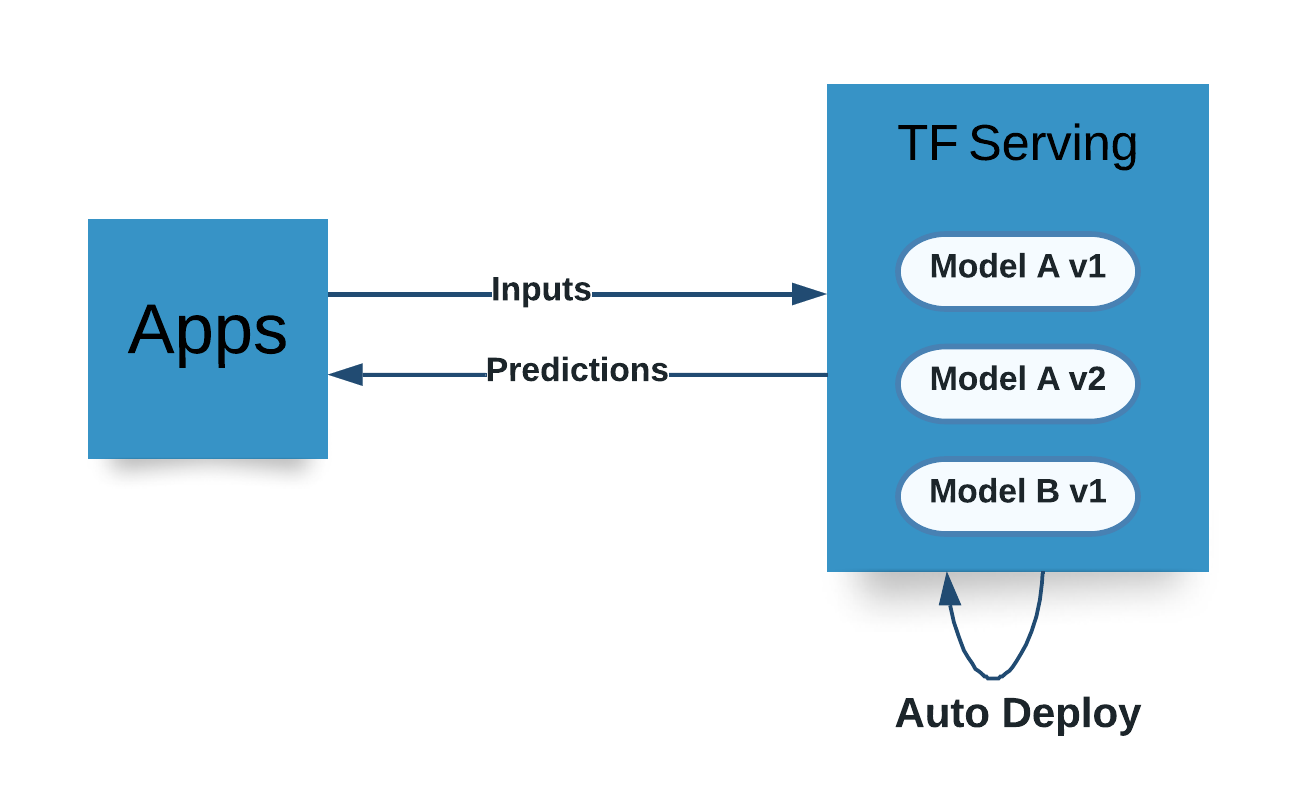
\includegraphics[width=0.8\textwidth]{figures/serving.png}
    \label{fig:serving}
\end{figure}

As introduced in section \ref{Micro-service Architecture} instead of building the micro-service from scratch and reinvent the wheel, we can use Tensorflow Serve. \enquote{A very efficient, battle-tested model server that can sustain a high load, serve multiple versions of your models and watch a model repository to automatically deploy the latest versions}, as Figure~\ref{fig:serving} shows~\cite{handsOnMachine}.

To use this functionality we first need set up some sort of file system structure to save our models and its versions. Using the function \textbf{\enquote{tf.saved\_model.save(model, path)}} we can easily serialize and save our model so it can be loaded by the Tensorflow Serve using the \textbf{\enquote{keras.models.load(model\_path)}} function. Models should be saved under the structure of \enquote{model name} and \enquote{version}, Figure~\ref{fig:model-save}. This will allow the server to auto-deploy all our models and expose them through an \gls{http} or \gls{grpc} endpoint.

\begin{figure}[h]
    \centering
    \caption{Save Keras Model File System Structure}
    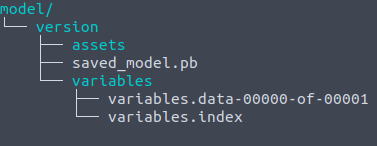
\includegraphics[width=0.75\textwidth]{figures/model-save.png}
    \label{fig:model-save}
\end{figure}

Tensorflow Serve can be easily downloaded from the Tensorflow's official repository. This will allow us to pull the image directly from the orchestrator, Listing~\ref{lst:docker-compose}. We only need to specify the ports which will be used by the REST/gRPC endpoints and mount the folder containing all of our models into our container, so the server knows where to find them. The request made to the http endpoint by the \gls{api} Gateway can be seen in Listing~\ref{lst:restApi/views.py}.

\subsection{Orchestration}

\gls{Docker} compose has been chosen for this project to orchestrate the different containers on the same host. Docker compose is a tool for defining and running multi-container Docker applications. With Compose, you use a \gls{YAML} file to configure your application’s services. Then, with a single command, you build and start all the services from your configuration. Docker compose has the following functionalities for managing the whole life cycle of your application:~\cite{dockerCompose}

\begin{itemize}
    \item Start, stop, and rebuild services.
    \item View the status of running services.
    \item Stream the log output of running services.
    \item Run a one-off command on a service.
\end{itemize}

Listing~\ref{lst:docker-compose} shows the docker compose file used to set up the orchestration configuration. Notice that the \gls{api} Gateway module depends on the other two modules to be initialized. 

\newpage
\begin{lstlisting}[language=python,caption=docker-compose.yaml,label={lst:docker-compose}]
version: "3.9"
services:
        apiGateway:
                image: marcosmartinezfco/tfg-api-gateway
                container_name: api-gateway
                networks:
                        - tfg-net
                ports:
                        - "8000:8000"
                depends_on:
                        - dataPipeline
        dataPipeline:
                image: marcosmartinezfco/tfg-data-pipeline
                container_name: data-pipeline
                networks:
                        - tfg-net
        predictionModule:
                image: tensorflow/serving
                container_name: prediction-module
                networks:
                        - tfg-net
                ports:
                        - "8501:8501"
                depends_on:
                        - dataPipeline
                volumes:
                        - ${MODELPATH}/mlp_model:/models/mlp_model
                environment:
                        - MODEL_NAME=mlp_model
networks:
        tfg-net:
                name: tfg-net
                driver: bridge
\end{lstlisting}

\section{Neural Network Definition}
\label{NN definition}

A key aspect of some types of \gls{ann} such as densely connected networks is that they have no memory. They process each input independently, without recording any state in between inputs. In contrast, as you are reading the present sentence, you are processing it word by word, while keeping memories of what came before.\cite{deepWithPython}

This lack of memory may present issues with any type of data that is time related or needs to keep a record of its past. \glspl{rnn} tackle this problem by iterating through the sequence elements and maintaining a state containing information relative to what it has seen so far. In essence, a \gls{rnn} is a type of \gls{ann} with an internal loop.

In this section we will walk through the development of a model capable of making predictions on stock prices using the historical time series of its price. But before trying to implement the model, we need to understand the problem, so that the whole process is easier. The following aspects need to be considered:

\begin{itemize}
    \item Understand what we are trying to predict and its business logic.
    \item Identify the type of problem we are dealing with.
    \item Define what and how to process the data.
\end{itemize}

It is obvious we are facing a regression problem since we are trying to predict a numeric value, the price. In regards to the business logic, we talked in section \ref{SoA:estado del arte} about how different features may have and impact on an asset's price. Along this chapter we will find out whether is possible to obtain good predictions just based on the past prices of an asset or if more features are needed to be taken into account.

\subsection{Data definition}

During the whole training process, only the historical data of Google will be used in the training for simplicity's sake. This data will be presented as a time series, as shown in Figure~\ref{fig:training-data}, containing the weekly or daily trading (depending of sample size requirements) information, i.e, the open price, close price, highest trading price, lowest trading price and the trading volume in dollars.

\begin{figure}[H]
    \centering
    \caption{Weekly Time Series of Google}
    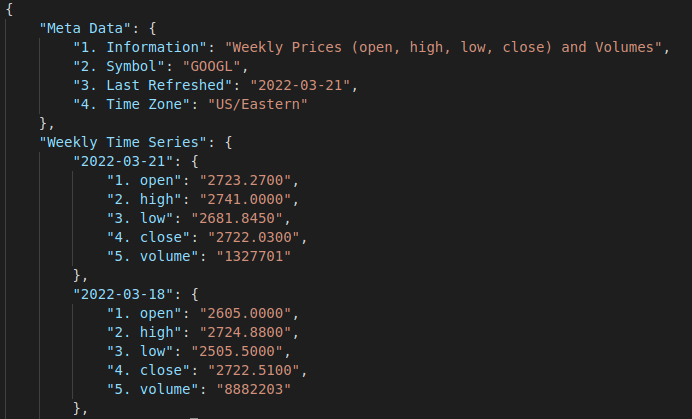
\includegraphics[width=0.8\textwidth]{figures/train data.png}
    \label{fig:training-data}
\end{figure}

Now we can easily transform our \gls{json} into a pandas data frame to easily manage information. Listing~\ref{lst:load-data} shows how to load the \gls{json} into our data frame with the date time as our index.

\begin{lstlisting}[language=python,caption=Load Data Into a Pandas Data Frame,label={lst:load-data}]
with open('./Training data/googl.json') as f:
    data = json.load(f)
raw_df = pd.DataFrame(data["Weekly Time Series"]).T
raw_df = raw_df.rename(lambda x: x.split(' ')[1], axis=1)
for c in raw_df.columns:
    raw_df[c] = pd.to_numeric(raw_df[c])
raw_df.index = pd.to_datetime(raw_df.index)
raw_df = raw_df.sort_index()
\end{lstlisting}

\subsection{Simple Interpolation Approach}

Now that we have all our training data prepared we can move on to the next step in the process, which is creating a basic model without artificial intelligence. It will give us a baseline point from which we can evaluate the most basic solution and why it may be interesting to use \gls{ai} algorithms.

\begin{lstlisting}[language=python,caption=Price Extrapolation,label={lst:base-model}]
def simple_predictions(df):
    success = 0
    forecast = []
    for x in range(3, len(df)-1):
        interpolate = interp1d(range(4), [(df.iloc[row]['open'] + df.iloc[row]['close']) / 2 for row in range(x-3, x+1)], kind='slinear', fill_value='extrapolate', bounds_error=False)
        forecast.append(t:=interpolate(4))
        if  df.iloc[x+1]['open'] <= t <= df.iloc[x+1]['close'] or df.iloc[x+1]['open'] >= t >= df.iloc[x+1]['close']:
            success += 1
    print(f'accuracy {success/(len(df)-4)*100}%')
\end{lstlisting}

We will build a prediction algorithm which will take into consideration the prices of the asset over the last month and its price trend, as Figure~\ref{fig:price-trend} shows, and interpolate a prediction linearly proportional to the trend. Listing~\ref{lst:base-model} shows a simple function that computes and test this approach, reaching 33.69\% accuracy in the whole data frame, Figure~\ref{fig:basic-acurracy} shows the accuracy for the last 40 weeks.

\begin{figure}[H]
    \centering
    \caption{Basic Price Trend}
    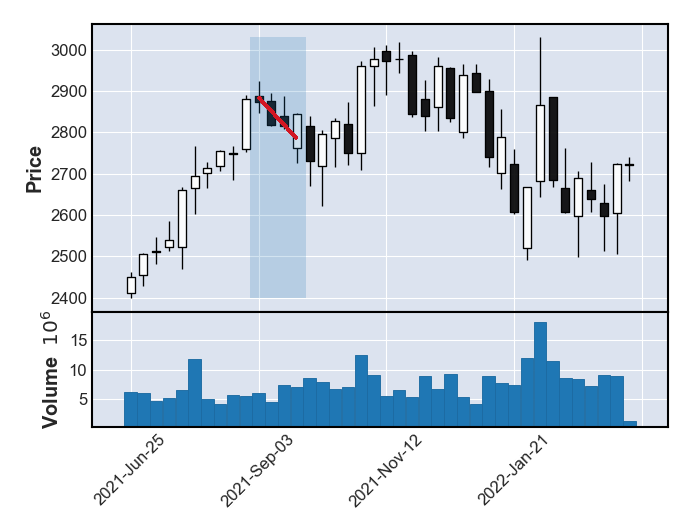
\includegraphics[width=0.7\textwidth]{figures/baselineCalc.png}
    \label{fig:price-trend}
\end{figure}

\begin{figure}[H]
    \centering
    \caption{Basic Model Accuracy, Last 40 Weeks}
    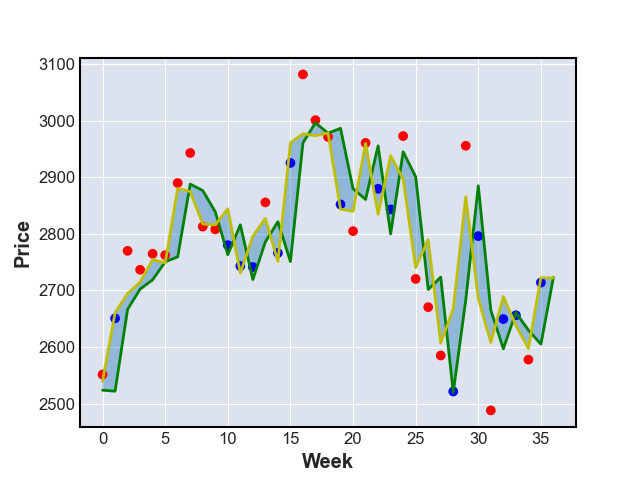
\includegraphics[width=0.7\textwidth]{figures/simple.png}
    \label{fig:basic-acurracy}
\end{figure}

\subsection{Multilayer Perceptron Approach}

Once we have a baseline model, let's find out if we can improve the prediction accuracy with a simple \gls{mlp}. Due to the small sample size of the weekly time series, daily time series data will be used for the deep learning algorithms instead. Listing~\ref{lst:perceptron} shows the assembly of the network. Figure~\ref{fig:perceptron} shows the accuracy obtained by the model in the test data set, reaching 31\%

\begin{lstlisting}[language=python,caption=\gls{mlp} Assembly,label={lst:perceptron}]
inputs = keras.Input(shape=(5,))
x = keras.layers.Dense(5, activation="relu")(inputs)
x = keras.layers.Dense(6, activation="relu")(x)
x = keras.layers.Dense(3, activation="relu")(x)
output = keras.layers.Dense(1, activation="linear")(x)
model = keras.Model(inputs=inputs, outputs=output, name="MLP")
model.compile(
    loss=keras.losses.MeanSquaredError(),
     optimizer=keras.optimizers.Adam(learning_rate=0.00001),
)
\end{lstlisting}

\begin{figure}[H]
    \centering
    \caption{\gls{mlp} Accuracy Over the Last 100 Days}
    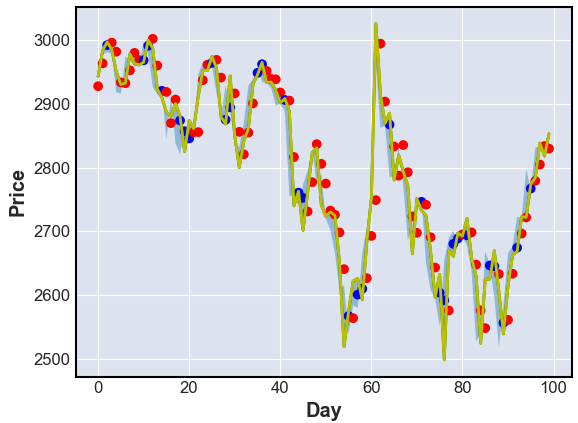
\includegraphics[width=0.7\textwidth]{figures/mlp.png}
    \label{fig:perceptron}
\end{figure}

After multiple hyper-parameter tunings~\footnote{\url{https://xkcd.com/1838/}}, it has been quite normal for the model to overfit and ending up giving the same prediction regardless of the input value. The final conclusion is that the model is unable to learn any correlation in price, given the input features, due to its simplicity. It tried to learn an average value for which the loss could be minimized rather than trying to recognize patterns in the data. That same value it was giving repeatedly could be that average value.

\subsection{Recurrent Neural Network Approach}

In section \ref{Artificial Intelligence} we talked about how \glspl{rnn} can keep an internal state and remember patterns inside our data. We will try now to build a simple model to see if we can improve the lack of memory seen in previous approaches.

First we need to prepare the information we are going to feed to the model. The weekly trading history of GOOGLE contains less than 800 samples which is quite little information. To solve this problem we take the daily trading history of the company and squeeze the data into weeks, Listing~\ref{lst:time-steps}, so now we have around 800 samples with 5 time steps each, shape (786,5,5) at the time of writing.

\begin{lstlisting}[language=python,caption=Week Time Steps GOOGLE,label={lst:time-steps}]
def week_batch_generator(raw, scaler):
    raw_df = scaler.transform(raw)
    df_x = raw_df[:-1]
    df_y = np.array([(x[0]+x[3])/2 for x in raw_df[1:]])
    x_batch = df_x[:-(len(df)%5)].reshape((len(df_x)//5, 5, 5)) 
    y_batch = df_y[:-(len(df)%5)].reshape(len(df_y)//5, 5, -1)
    return (x_batch[:-100], y_batch[:-100]), (x_batch[-100:], np.array(raw_df[1:-(len(df)%5),[0, 3]][-100:]))
\end{lstlisting}

During training we have used two different callbacks. These are objects that can perform actions at various stages of training, e.g, at the start or end of an epoch or before or after a single batch. First, we have the \textbf{\enquote{EarlyStopping}} class which allows to stop training when a given metric shows no improvement, like training loss in this particular case. Second, we have implemented a custom callback class which allows to see graphic representation of the training and validation loss during in real time during training, Listing~\ref{lst:callback}. These callbacks are added to the network configuration as shown in Listing~\ref{lst:lstm-assembly}.

\begin{lstlisting}[language=python,caption=Custom Keras Callback,label={lst:callback}]
Created with the help of Rubén Rincón Blanco
class MyCallback(keras.callbacks.Callback):
    def on_epoch_end(self, epoch, logs = None):
        plt.rcParams["figure.figsize"] = (30,10)
        fig, ax = plt.subplots()
        fig.suptitle(f"epoch: {epoch}, {logs}")
        history = list(logs.keys())
        for key in history:
            if key not in self.valores:
                self.valores[key] = []
            self.valores[key].append(logs[key])
            ax.plot(self.valores[key], label = key, c = colors[0 if "loss" in key else 1], linestyle='--' if 'val' in key else '-')
            ax.legend(loc = "upper right" if "loss" in key else "upper left")
        plt.show()
        display.clear_output(wait = True)
    def __init__(self):
        self.valores = {}
    def on_train_end(self, logs = None):
        print(f"Finished: {logs}")
\end{lstlisting}

\begin{lstlisting}[language=python,caption=\gls{lstm} Assembly,label={lst:lstm-assembly}]
inputs = keras.layers.Input(shape=(x_train.shape[1:]))
x = keras.layers.LSTM(3, activation=keras.layers.LeakyReLU() , return_sequences=True)(inputs)
x = keras.layers.Dropout(0.2)(x)
x = keras.layers.LSTM(2, activation=keras.layers.LeakyReLU() , return_sequences=False)(x)
x = keras.layers.Dropout(0.2)(x)
output = keras.layers.Dense(1, activation='linear')(x)
model_lstm = keras.Model(inputs=inputs, outputs=output, name="v1.0")
model_lstm.compile(
    loss=keras.losses.MeanSquaredError(),
    optimizer=keras.optimizers.Adam(learning_rate=0.00001),
)
history = model_lstm.fit(
    x_train[:-100], y_train[:-100],
    validation_data=(x_train[-100:], y_train[-100:]), 
    batch_size=32, epochs=100, shuffle=False,
    verbose=0,
    callbacks=[
        keras.callbacks.EarlyStopping(patience=15, restore_best_weights=True),
        MyCallback()
    ]
)
\end{lstlisting}

\begin{figure}
    \centering
    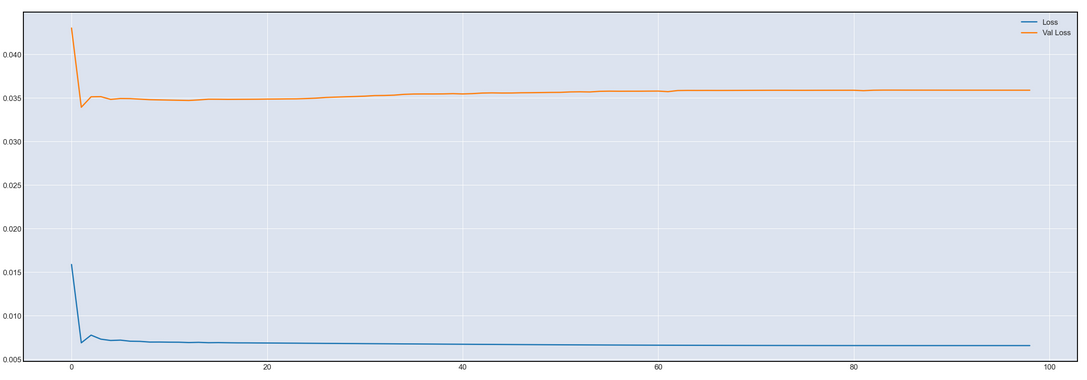
\includegraphics[width=\textwidth]{figures/loss-lstm.png}
    \caption{\gls{lstm} Training Loss}
    \label{fig:loss-lstm}
\end{figure}

As in the previous section, the \gls{lstm} model presents high levels of overfitting, Figure~\ref{fig:loss-lstm} . It also presents huge sings of mode collapse\footnote{When model can only produce a single type of output or a small set of outputs regardless of the input data.} within the average price range of the trading history, as seen with the \gls{mlp} model, regardless of the hyper-parameters configuration. 


